\documentclass[preview,border=4mm,convert={convertexe={magick},outext=.ps}]{standalone}
\usepackage[dvipdfm]{geometry}

%graphics
\usepackage{xcolor}
\usepackage{tikz}
\usetikzlibrary{shapes.geometric, shapes.multipart, arrows, arrows.meta,calc, through,intersections, circuits.logic.US}
\usepackage[caption=false,font=footnotesize]{subfig}

\colorlet{dot-color}{black!80}
\tikzset{
    pics/cell/.style = {
        code = {%
        \coordinate (-center) at (0,0);
        
        \fill +(-0.55,-0.55) coordinate(-sw) 
           -- +(-0.55, 0.55) coordinate(-nw)
           -- +( 0.55, 0.55) coordinate(-ne)
           -- +( 0.55,-0.55) coordinate(-se)
           -- cycle;
        \coordinate (-swo) at ($ (-center)!0.5!(-sw) $);
        \coordinate (-nwo) at ($ (-center)!0.5!(-nw) $);
        \coordinate (-neo) at ($ (-center)!0.5!(-ne) $);
        \coordinate (-seo) at ($ (-center)!0.5!(-se) $);
        
        \coordinate (-south) at ($ (-sw)!.5!(-se) $);
        \coordinate (-north) at ($ (-nw)!.5!(-ne) $);
        \coordinate (-west)  at ($ (-sw)!.5!(-nw) $);
        \coordinate (-east)  at ($ (-se)!.5!(-ne) $);
        
        \fill[white] (-swo) let \p1=($ (-center)!.5!(-swo) $) in circle ({veclen(\x1,\y1)});
        \fill[white] (-nwo) let \p1=($ (-center)!.5!(-nwo) $) in circle ({veclen(\x1,\y1)});
        \fill[white] (-neo) let \p1=($ (-center)!.5!(-neo) $) in circle ({veclen(\x1,\y1)});
        \fill[white] (-seo) let \p1=($ (-center)!.5!(-seo) $) in circle ({veclen(\x1,\y1)});
        
        \ifnum#1=1\relax
            \fill[dot-color] (-swo) let \p1=($ (-center)!.32!(-swo) $) in circle ({veclen(\x1,\y1)});
            \fill[dot-color] (-neo) let \p1=($ (-center)!.32!(-neo) $) in circle ({veclen(\x1,\y1)});
        \else
            \ifnum#1=-1\relax
                \fill[dot-color] (-nwo) let \p1=($ (-center)!.32!(-nwo) $) in circle ({veclen(\x1,\y1)});
                \fill[dot-color] (-seo) let \p1=($ (-center)!.32!(-seo) $) in circle ({veclen(\x1,\y1)});
            \else
                \fill[dot-color] (-swo) let \p1=($ (-center)!.22!(-swo) $) in circle ({veclen(\x1,\y1)});
                \fill[dot-color] (-nwo) let \p1=($ (-center)!.22!(-nwo) $) in circle ({veclen(\x1,\y1)});
                \fill[dot-color] (-neo) let \p1=($ (-center)!.22!(-neo) $) in circle ({veclen(\x1,\y1)});
                \fill[dot-color] (-seo) let \p1=($ (-center)!.22!(-seo) $) in circle ({veclen(\x1,\y1)});
            \fi
        \fi
        }
    },
    pics/cell/.default={0}
}

\definecolor{clock0}{RGB}{89,89,91}
\definecolor{clock1}{RGB}{129,130,132}
\definecolor{clock2}{RGB}{210,210,212}
\definecolor{clock3}{RGB}{168,169,173}
\definecolor{input}{RGB}{230,230,230}
\definecolor{output}{RGB}{40,40,40}
\definecolor{fixed}{HTML}{000000}

\begin{document}
\begin{figure}[!t]
\centering

\subfloat[Logic Network]{
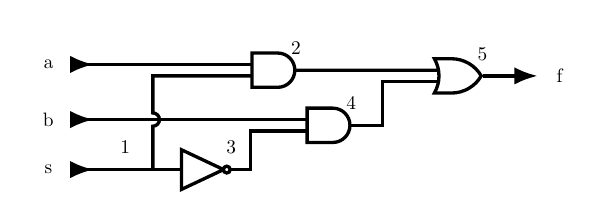
\begin{tikzpicture}[transform shape, scale=0.7, circuit logic US, every node/.style={very thick, minimum size=0.75cm}, very thick]

\node(o1)[or gate, point right]  at (6,3){};
\draw[>=Latex, ->] (o1.output) node[above]{5} -- +(1,0) node[right]{f};

\node (a1)[and gate, point right] at ($(o1.input 1) - (3,0)$) {};
\node at (a1.output)[above]{2};
\node (a2)[and gate, point right] at ($(o1.input 1) - (2,1)$) {};
\node at (a2.output)[above]{4};

\draw (o1.input 1) -- (a1.output);
\draw (o1.input 2) -- ++(-1,0) |- (a2.output);

\node (n1)[not gate, point right] at ($(a2.input 2) - (2,0.7)$) {};
\node at (n1.output)[above]{3};
\draw (a2.input 2) -- ++(-1, 0) |- (n1.output);

\coordinate (pivot) at ($(n1.input) - (2,0)$);

\begin{scope}[>=Latex]
\draw[>-] (n1.input -| pivot) node(s)[left]{s} -- node[above]{1}(n1.input);
\draw[>-] (a2.input 1 -| pivot) node(b)[left]{b} --(a2.input 1);
\draw[>-] (a1.input 1 -| pivot) node(a)[left]{a} --(a1.input 1);
\end{scope}

\coordinate (p2) at ($(n1.input) - (0.5, 0)$);
\coordinate (arcc) at (p2 |- b);
\draw (p2)  -- ($(arcc) - (0, 0.12) $) arc[start angle=-90, end angle=90, radius=0.12] |- (a1.input 2);
\end{tikzpicture}
}
\subfloat[Node Placement]{
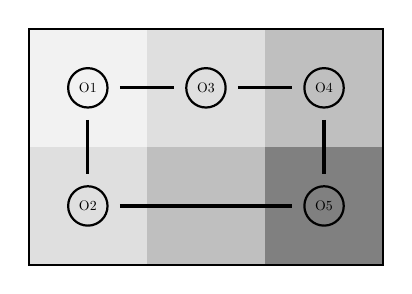
\begin{tikzpicture}[transform shape, scale=0.5]
\fill[lightgray!20] (0,3) rectangle (3,6);
\fill[lightgray!50] (0,0) rectangle (3,3);
\fill[lightgray!50] (3,3) rectangle (6,6);
\fill[lightgray] (3,0) rectangle (6,3);
\fill[lightgray] (6,3) rectangle (9,6);
\fill[gray] (6,0) rectangle (9,3);
\draw[thick] (0,0) rectangle (9,6);

\begin{scope}[every node/.style={circle, draw, thick, minimum size=1cm}]
    \node(O1) at (1.5, 4.5) {O1};
    \node(O2) at (1.5, 1.5) {O2};
    \node(O3) at (4.5, 4.5) {O3};
    \node(O4) at (7.5, 4.5) {O4};
    \node(O5) at (7.5, 1.5) {O5};
\end{scope}

\begin{scope}[very thick]
    \draw ($(O1.east) + (0.3,0)$) -- ($(O3.west) - (0.3,0)$);
    \draw ($(O3.east) + (0.3,0)$) -- ($(O4.west) - (0.3,0)$);
    \draw ($(O1.south) - (0,0.3)$) -- ($(O2.north) + (0, 0.3)$);
    \draw ($(O4.south) - (0,0.3)$) -- ($(O5.north) + (0, 0.3)$);
    \draw ($(O2.east) + (0.3,0)$) -- ($(O5.west) - (0.3,0)$);
\end{scope}
\end{tikzpicture}
}

\subfloat[Gate Level Placement]{
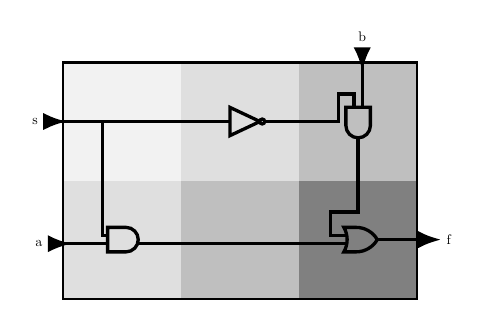
\begin{tikzpicture}[transform shape, scale=0.5]
\fill[lightgray!20] (0,3) rectangle (3,6);
\fill[lightgray!50] (0,0) rectangle (3,3);
\fill[lightgray!50] (3,3) rectangle (6,6);
\fill[lightgray] (3,0) rectangle (6,3);
\fill[lightgray] (6,3) rectangle (9,6);
\fill[gray] (6,0) rectangle (9,3);
\draw[thick] (0,0) rectangle (9,6);

\begin{scope}[circuit logic US, every node/.style={very thick, minimum size=1cm}]
    \node(and1)[and gate, point right] at (1.5, 1.5) {};
    \node(not1)[not gate, point right] at (4.5, 4.5) {};
    \node(and2)[and gate, point down] at (7.5, 4.5) {};
    \node(or1)[or gate, point right] at (7.5, 1.5) {};
\end{scope}

\begin{scope}[>=Latex, very thick]
\draw[>-] ($(and1.input 2) - (1.5,0)$) node[left]{a} -- (and1.input 2);
\draw[>-] (-0.5, 4.5) node[left]{s} -- (not1.input);
\draw (1, 4.5) |- (and1.input 1);

\draw (not1.output) -- (7,4.5) -- ++ (0,0.7) -| (and2.input 2);
\draw[>-] ($(and2.input 1) + (0, 1.5)$) node[above]{b}  -- (and2.input 1);
\draw (and2.output) -- (7.5, 2.2) -- ++(-0.7, 0) |- (or1.input 1);

\draw (or1.input 2) -- ++(-5.3,0) ;
\draw[->] (or1.output) -- ++(1.6,0) node[right]{f};
\end{scope}
\end{tikzpicture}
}
\hfil
\subfloat[Cell Level Placement]{
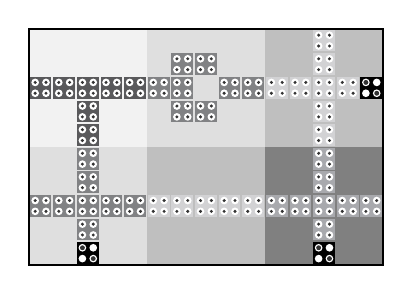
\begin{tikzpicture}[transform shape, scale=0.5]
\fill[lightgray!20] (0,3) rectangle (3,6);
\fill[lightgray!50] (0,0) rectangle (3,3);
\fill[lightgray!50] (3,3) rectangle (6,6);
\fill[lightgray] (3,0) rectangle (6,3);
\fill[lightgray] (6,3) rectangle (9,6);
\fill[gray] (6,0) rectangle (9,3);
\draw[thick] (0,0) rectangle (9,6);

\begin{scope}[scale=0.5]

%input s
\pic [clock0] at (0.6, 9) {cell};
\pic [clock0] at (1.8, 9) {cell};
\pic [clock0] at (3, 9) {cell};
\pic [clock0] at (4.2, 9) {cell};
\pic [clock0] at (5.4, 9) {cell};

\pic [clock0] at (3, 7.8) {cell};
\pic [clock0] at (3, 6.6) {cell};
%inverter
\pic [clock1] at (6.6, 9) {cell};
\pic [clock1] at (7.8, 9) {cell};
\pic [clock1] at (7.8, 10.2) {cell};
\pic [clock1] at (9, 10.2) {cell};
\pic [clock1] at (7.8, 7.8) {cell};
\pic [clock1] at (9, 7.8) {cell};
\pic [clock1] at (10.2, 9) {cell};
\pic [clock1] at (11.4, 9) {cell};

%and gate b
\pic [clock2] at (12.6, 9) {cell};
\pic [clock2] at (13.8, 9) {cell};
\pic [clock2] at (15, 9) {cell};
\pic [clock2] at (16.2, 9) {cell};
\pic [fixed] at (17.4, 9) {cell=-1};

\pic [clock2] at (15, 11.4) {cell};
\pic [clock2] at (15, 10.2) {cell};
\pic [clock2] at (15, 7.8) {cell};
\pic [clock2] at (15, 6.6) {cell};

%and gate a
\pic [clock1] at (0.6, 3) {cell};
\pic [clock1] at (1.8, 3) {cell};
\pic [clock1] at (3, 3) {cell};
\pic [clock1] at (4.2, 3) {cell};
\pic [clock1] at (5.4, 3) {cell};

\pic [clock1] at (3, 5.4) {cell};
\pic [clock1] at (3, 4.2) {cell};
\pic [clock1] at (3, 1.8) {cell};
\pic [fixed] at (3, 0.6) {cell=-1};

%strait line
\pic [clock2] at (6.6, 3) {cell};
\pic [clock2] at (7.8, 3) {cell};
\pic [clock2] at (9, 3) {cell};
\pic [clock2] at (10.2, 3) {cell};
\pic [clock2] at (11.4, 3) {cell};

%or gate f
\pic [clock3] at (12.6, 3) {cell};
\pic [clock3] at (13.8, 3) {cell};
\pic [clock3] at (15, 3) {cell};
\pic [clock3] at (16.2, 3) {cell};
\pic [clock3] at (17.4, 3) {cell};

\pic [clock3] at (15, 5.4) {cell};
\pic [clock3] at (15, 4.2) {cell};
\pic [clock3] at (15, 1.8) {cell};
\pic [fixed] at (15, 0.6) {cell=-1};

\end{scope}
\end{tikzpicture}
}

\end{figure}
\end{document}
